%*******10********20********30********40********50********60********70********80

% For all chapters, use the newdefined chap{} instead of chapter{}
% This will make the text at the top-left of the page be the same as the chapter

\chap{AuthorVis: A Co-authorship Visualization and Scientific Collaboration Prediction tool}
\label{chap_authorvis}
\section{Background}
In this chapter, we describe a co-authorship network exploration, and link prediction tool we created and that is specific to the three networks investigated in this dissertation. While many network visualization solutions have already been proposed, most of them are not specifically adapted to co-authorship networks \cite{nakazono_nel_2006,odoni_visualisation_2017,liu_toolkits_2004,horak_forcoa.net:_2011}. 
% New citation to add: nakazono_nel_2006,odoni_visualisation_2017,liu_toolkits_2004,horak_forcoa.net:_2011,mena-chalco_brazilian_2014
Even those designed for visualizing co-authorship networks have several limitations among others, their inability to satisfactorily display large networks, the lack of interactivity in the display, and the inability for the end user to control the display \cite{nakazono_nel_2006}.\\
Here, we present a tool that not only addresses those limitations, but provides a visualization of each of the networks and allows the end user to query each network. Our approach integrates bibliometrics information to the visualization. In our design model, all the authorship information are embedded within the display of the network. %, and at the fingertip of the end user. 
%We also provide a link prediction/recommendation tool to allow the users to predict future collaborations and recommend new ones. 
In the visualization interface, users can select a particular node or author to emphasize its subnetwork, hover over a node to display author's information or select an edge between two vertices/authors to display information related to materials co-authored by the two vertices defining that particular edge. 

%\section{Related work}
%Various authors have proposed diverse tools for the visualizations of co-authorship networks. One of such tools has been reported by Liu and colleagues \cite{liu_toolkits_2004} who proposed an author navigator application for visual examination of co-authorhip networks. In their conception of the toolkits, the authors combined a web based application tool for the interactive navigation of the network and a Java based backend swing application for the management of CGI requests. To support Brazilian researchers, Barbosa and colleagues proposed \textbf{VRRC}, a web based tool for the visualization and recommendation of co-authorship network \cite{barbosa_vrrc:_2012}. According to its developers, \textbf{VRRC} provides an interactive visualization, an overview of the collaborations over time, and recommendations to initiate new collaborations and reinforce existing ones. \textbf{VICI}, another co-authorship visualization tool was proposed by  Odoni and colleagues \cite{odoni_visualisation_2017}. \textbf{VICI} combined a Python based backend system for the extraction and management of the network data and a web based frontend using Flask \cite{grinberg_flask_2014} to display the network. The visualization of the network was finally rendered using the Javascript D3.js \cite{bostock_d3._2012} library. \textbf{NeL$^2$}, a general purpose tool for the visualization of networks as a layered network diagram was proposed by Nakazono, Misue, and Tanaka \cite{nakazono_nel_2006}. They applied their tool to the visualization of co-authorship networks to visualize transitions in the network over a period of time, as well as various co-authorship data. \\
%Another framework, the WebRelievo system was proposed for the visualization of the evolutionary processes of Web pages \cite{toyoda_system_2005}. Other techniques were also proposed for the visualization of co-citation networks \cite{chen_visualizing_1999}, and for the visualization of the relationship of scientific literature \cite{erten_simultaneous_2005}. \\
%Here, we propose \textbf{AuthorVis}, a co-authorship visualization and scientific collaboration tool for Malaria, TB and HIV/AIDS research in Benin. In addition to providing the same features as the aforementioned tools, with \textbf{AuthorVis}, we propose a different approach to co-authorship network visualization. Our approach integrates network structure and network data, hence requires no data management using traditional database framework. In addition, our visualization allows the end-user to navigate the network with an interactive navigation panel, but also integrate published materials within the visualization interface.

\section{Data}
Currently, \textbf{AuthorVis} is designed specifically for the visualization of the Malaria, Tuberculosis and HIV/AIDS collaborative network in Benin. We refer the reader to section \ref{sec:data_collection} for details on the collection and treatment of the co-authorship data. On the server end, each network data is maintained as an igraph object. Each submitted user query is interpreted and incorporated in an igraph function to extract the network data. Another igraph object is generated as a result and converted into a JSON data using an executable Python script that we provided within the tool.

\section{Programmer View}
\subsection{Design and Architecture}
%We propose a co-authorship visualization and scientific collaboration tool for Malaria, TB and HIV/AIDS research in Benin. In addition to providing the same features as the aforementioned tools, we propose a different approach to co-authorship network visualization. Our approach integrates network structure and network data, hence requires no data management using traditional database framework. In addition, our visualization allows the end-user to navigate the network with an interactive navigation panel, but also integrates published materials within the visualization interface.
\textbf{AuthorVis} is implemented as a Shiny dashboard with an R based backend system that manages each co-authorship network data as an igraph object \cite{csardi_igraph_2006}. The backend server side is a combination of a Shinyserver and an HTTP server (Figure \ref{av_design}). The Shiny application is built using the \textbf{Shinyboard} \cite{chang_shiny:_2017,chang_shinydashboard:_2015} R package. A set of R scripts manages global libraries (\texttt{global.R}), controls the dashboard user interface (\texttt{ui.R}), and handles backend processings (\texttt{server.R}). The user interface script (\texttt{ui.R}) communicates with the frontend dashboard interface on the client side and the backend processing script (\texttt{server.R}) on the Shinyserver. When the user submits a request, it is passed from the dashboard interface to \texttt{server.R} via \texttt{ui.R}. The request is subsequently processed, and the output is transferred to the dashboard on the client side via \texttt{ui.R}. However, when the request is a query to explore and visualize a co-authorship network, the server also outputs a graph object which is converted into JSON graph file thanks to a python script. The graph file is then transferred to the HTTP server to be displayed on the Network Visualization Interface. The HTTP server has been implemented with the \href{https://nodejs.org}{Node.js} built-in HTTP module. Node.js is a Javascript server-side platform for the development of web servers \cite{WilsonNodejsRight2018}. The front-end Network Visualization Interface is handled by the HTTP web server which renders the JSON graph object into an HTML file (\texttt{index.html}). A script (\texttt{code.js}) written in Javascript using the Javascript D3.js \cite{bostock_d3._2012} library handles user interactivity and the control of the display. D3.js or Data-Driven Documents has been designed for manipulating documents based on data and to generate interactive and dynamic data visualizations in web browsers (Figure \ref{av_design}).
% processes the query submitted by the end user through the dashboard. It is combined to a Javascript web based frontend that displays the network graph, and handle user interactions with the network. Figure \ref{authorvis_screen1} displays the network query and exploration interface (on top) and the link prediction interface (on the bottom). The network query and exploration interface is accessible from the side bar menu "Explore Network" and the link prediction interface is accessible via the side bar menu "Prediction". Other options in the side bar menu include the "Codes" menu where we share the Shiny dashboard script, the "Readme" menu displaying a documentation for the tool, and the "About" menu which provides general information on the tool.

%\begin{figure}[!ht]
%\centering
%\hspace{-1.5cm}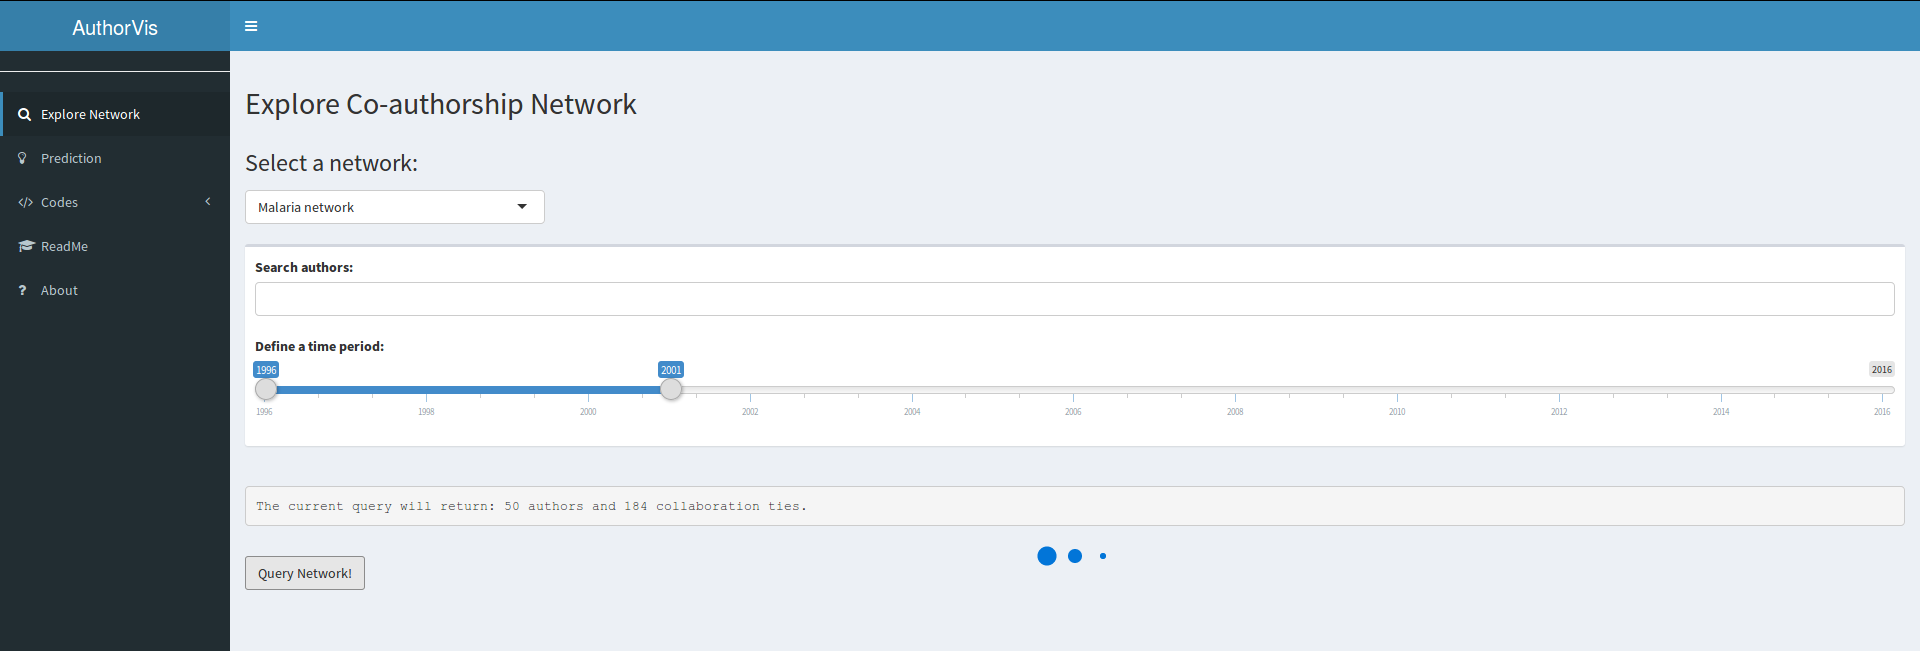
\includegraphics[scale=0.26]{Chapters/authorvis/screen2}
%~\\~\\
%\hspace{-1.5cm}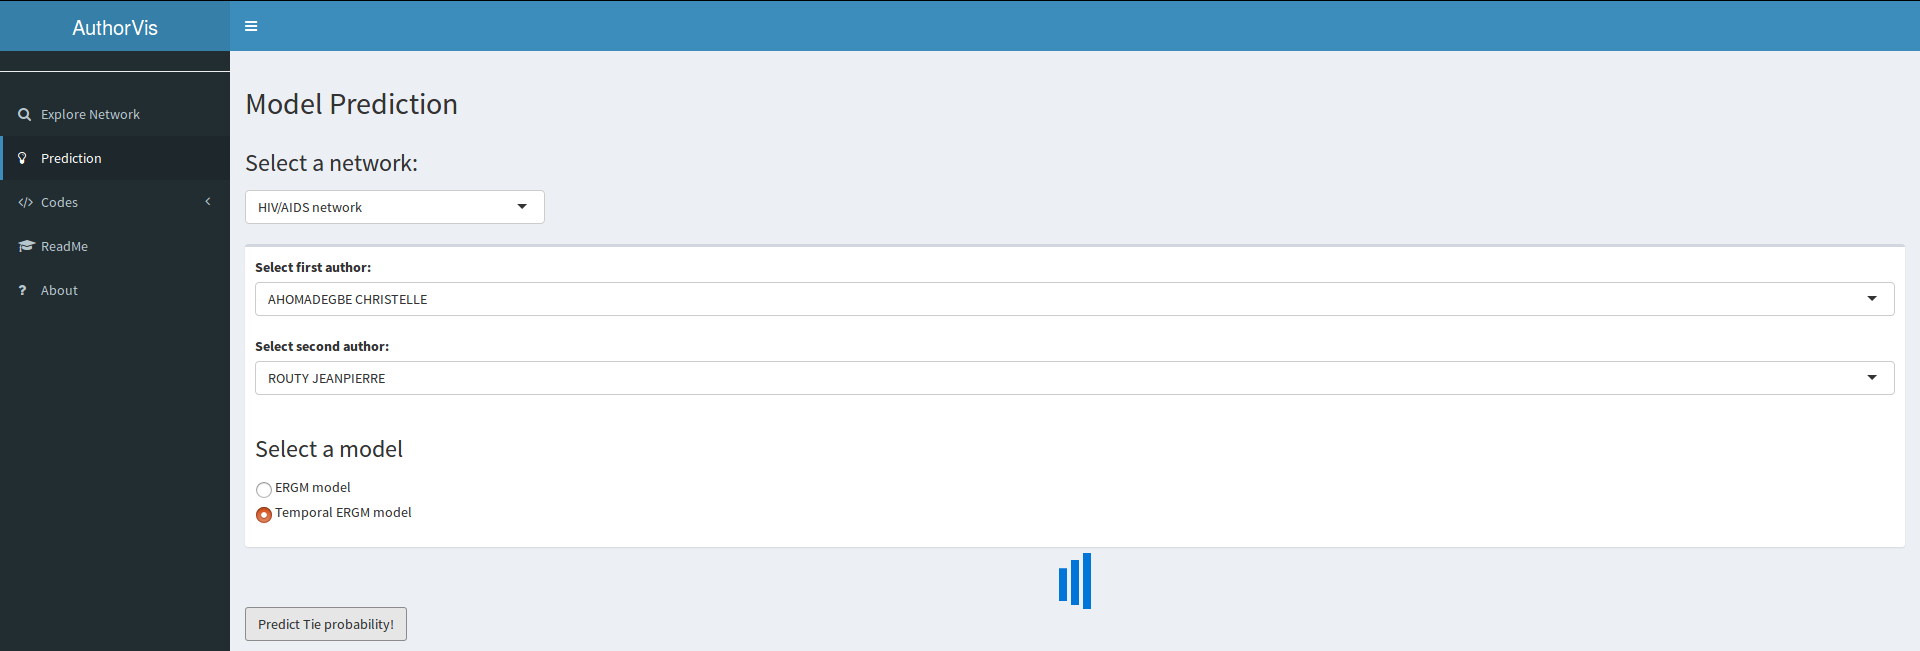
\includegraphics[scale=0.26]{Chapters/authorvis/screen4}
%\caption{Screenshots of the Shiny application interface displaying the network exploration interface (top), and the link prediction interface (bottom).}
%\label{authorvis_screen1}
%\end{figure}
%\pagebreak
\begin{sidewaysfigure}
\centering
%\begin{sidewaysfigure}
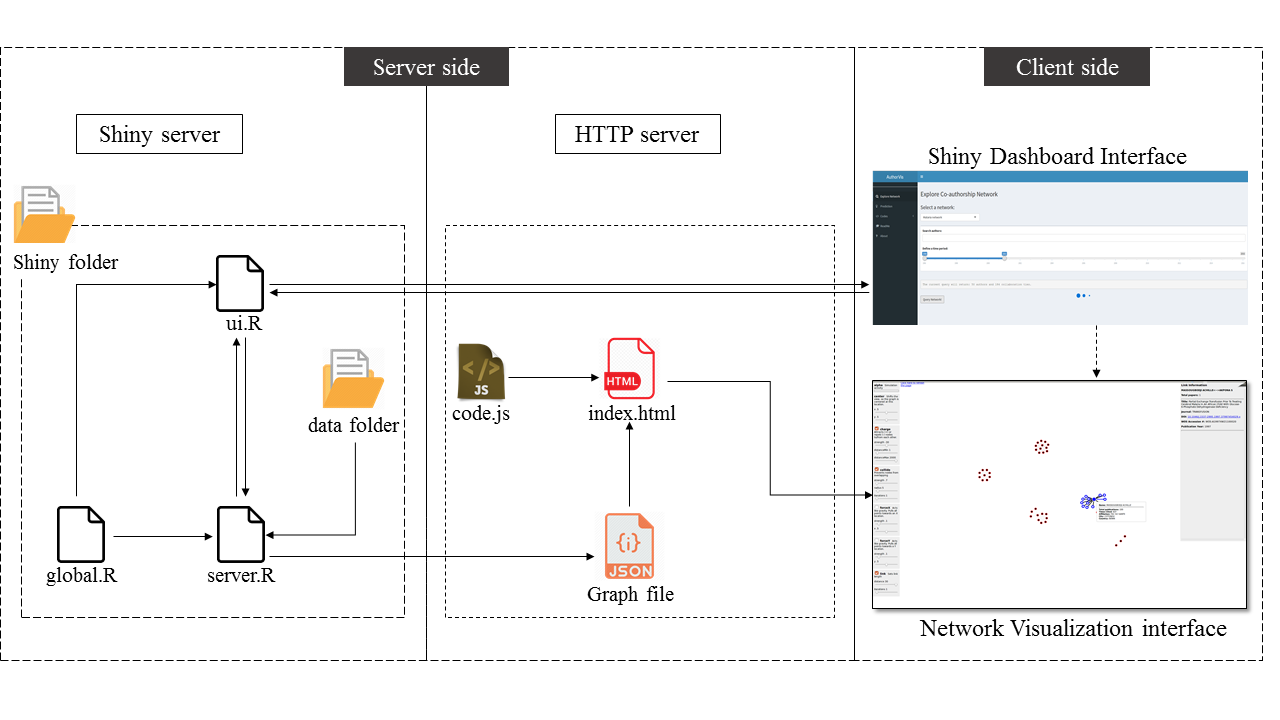
\includegraphics[scale=0.68, trim={0 2cm 0.5cm 2cm}]{Chapters/authorvis/programmerView}
%\end{sidewaysfigure}
\caption{Authorvis Design and Architecture}
\label{av_design}
%\end{figure}
\end{sidewaysfigure}
%
%\subsection{Web Framework}

\section{User View}
\subsection{Shiny Dashboard Interface}
The frontend Shiny dashboard interface has five menu options displayed on its left sidebar. The network query and exploration interface is accessible from the "Explore Network" menu option and the link prediction interface is accessible via the "Prediction" menu option. Other options in the side bar menu include the "Codes" menu where we share the Shiny dashboard scripts, the "Readme" menu displaying a documentation for the tool, and the "About" menu which provides general information on the tool (See subfigure (d) on figure \ref{av_userView}).\\
When the user selects the "Explore Network" menu option, the dashboard brings him to the appropriate page containing a simple query builder. After selecting a network, the user can define a time period and may search for a specific author or set of authors. As the user builds his query, the dashboard responds interactively, displaying the number of vertices and edges returned by the query. When the user clicks on the "Query Network!" button, the query is submitted to the server. Once the processing is done, a URL is displayed and the user is prompted to click on it to launch the Network Visualization Interface (subfigures (a) and (b) on figure \ref{av_userView}).\\
Figure \ref{net_vis} is a screenshot of the dashboard prediction page with its simple query builder. It is accessible via the "Prediction" menu option in the side bar. Here again, the user is prompted to select a network, a first and second authors, and choose a model. Upon click on the "Predict Tie Probability!" button, the query is submitted to the server. Once the processing is done, the output is sent back to the page for display. The prediction tool is model-based and used the final ERGMs and TERGMs from chapters \ref{chap:malaria}, \ref{chap:hiv}, and \ref{chap:tb} to calculate a micro-interpretation probability of collaboration between two authors \cite{desmarais_micro-level_2012}.

%\pagebreak
\begin{sidewaysfigure}
\centering
%\begin{sidewaysfigure}
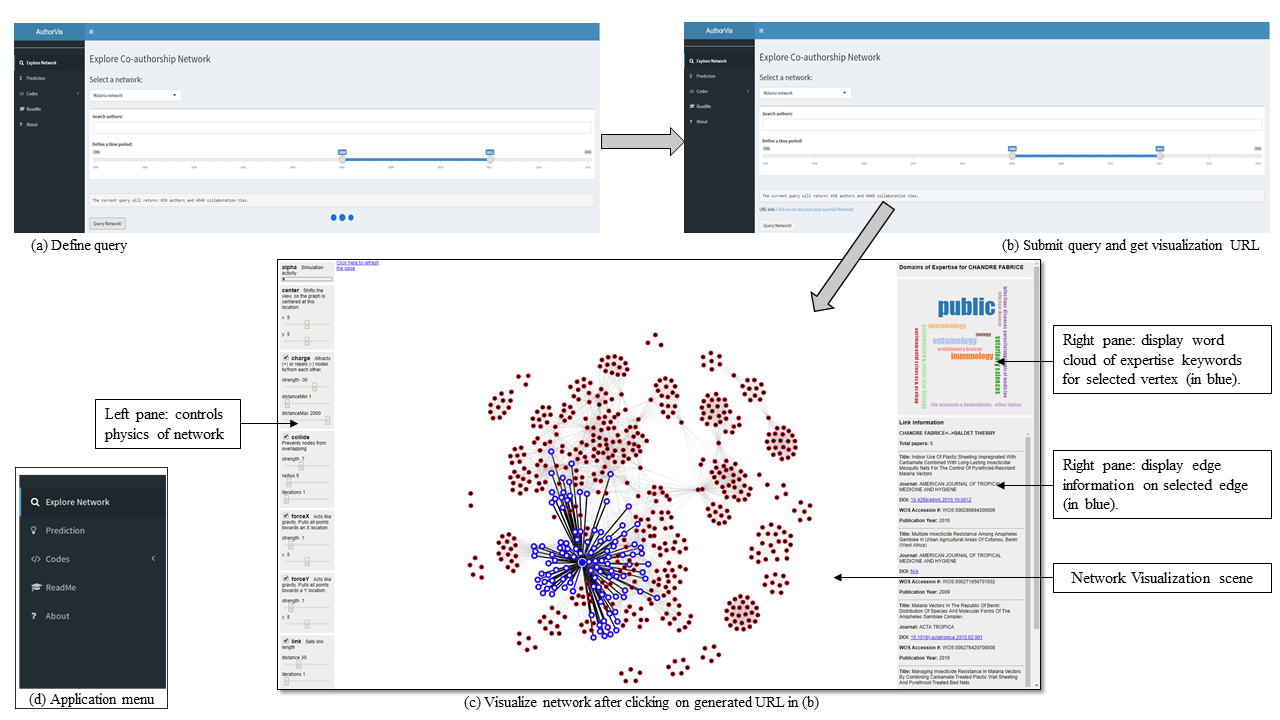
\includegraphics[scale=0.68]{Chapters/authorvis/userView2}
%\end{sidewaysfigure}
\caption{User View of the Authorvis co-authorship tool}
\label{av_userView}
%\end{figure}
\end{sidewaysfigure}

\begin{figure}[!ht]
\centering
\hspace{-1.5cm}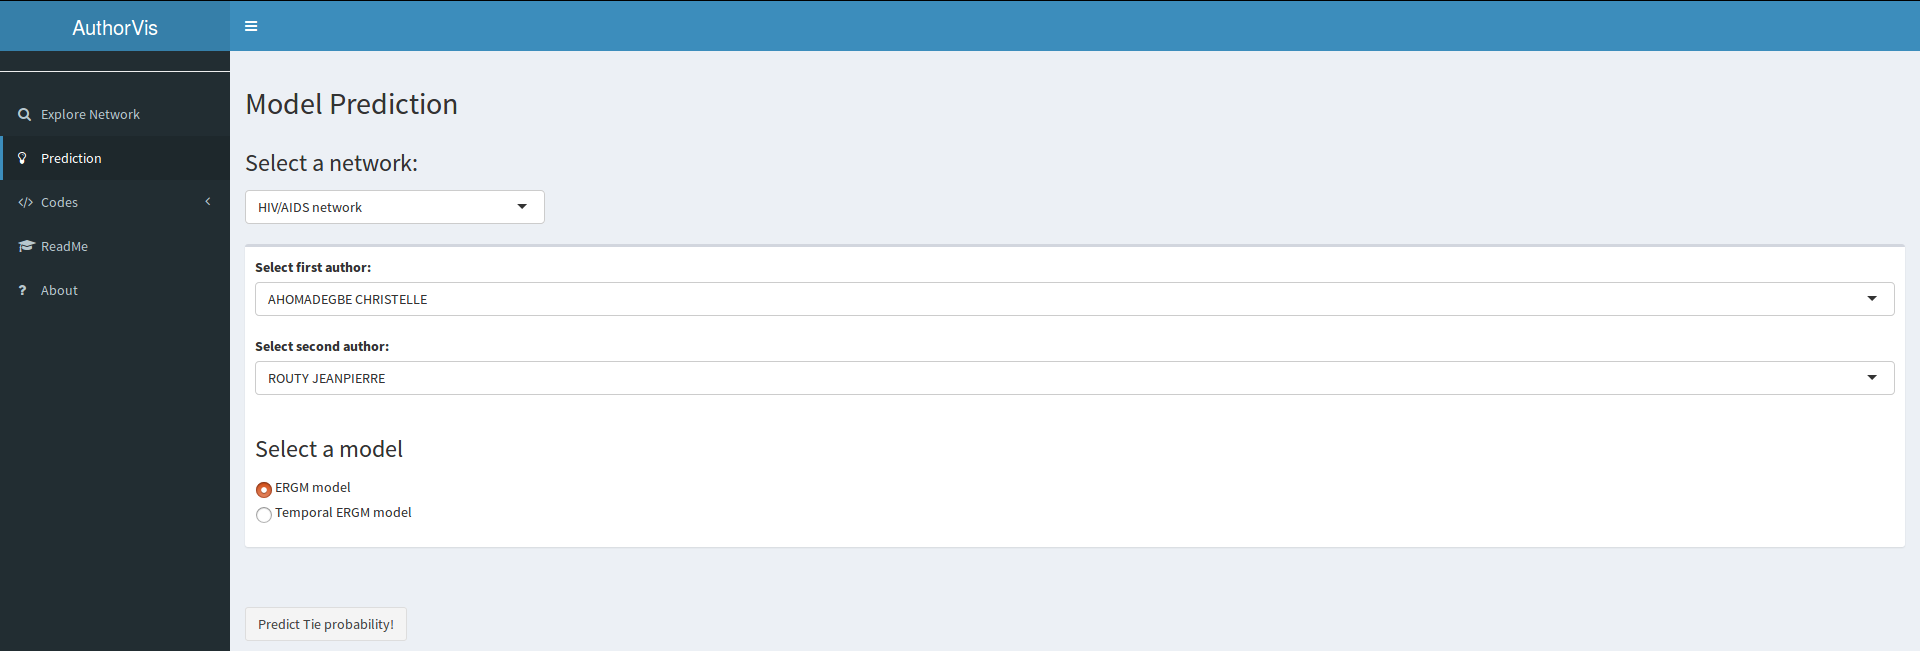
\includegraphics[scale=0.26]{Chapters/authorvis/screen3}
\caption{Screenshot of the co-authorship prediction page.}
\label{net_vis}
\end{figure}


\subsection{Network Visualization Interface}
The frontend Network Visualization Interface has three main parts: a left control pane, an SVG scene, and a right link information pane. The user can adjust the display of the network by modifying the default options of the physics of the network \cite{newman_physics_2008} using the control pane on the left. The SVG scene displays the queried network. In the SVG scene, a mouse hover over a vertex displays a tooltip of details on the author represented by the vertex, and a single click on a vertex displays a word cloud of the keywords expertise on that vertex, showing what the work of the vertex author is about. A double-click on a vertex highlights the subnetwork of the author represented by that specific vertex. Once an edge is clicked, its color turns blue and the list of published materials co-authored by the two vertices defining the clicked edge is displayed on the link information right pane. All published materials listed in the right pane can be traced back to their publication page on the web via their DOI or the WOS accession number with a single click (subfigure (d) on figure \ref{av_userView}).\\
%%%Added after corrections
\textbf{AuthorVis} can be used by policy makers to visualize collaboration interactions in time between researchers. Figure \ref{mostCited}, for example, depicts the co-authorship network of the 10 most cited papers in malaria research in Benin, highlighting one author (Prof. Martin AKOGBETO) as the most important author for the sustainability of the network.

\begin{figure}[!ht]
\centering
\hspace{-1.5cm}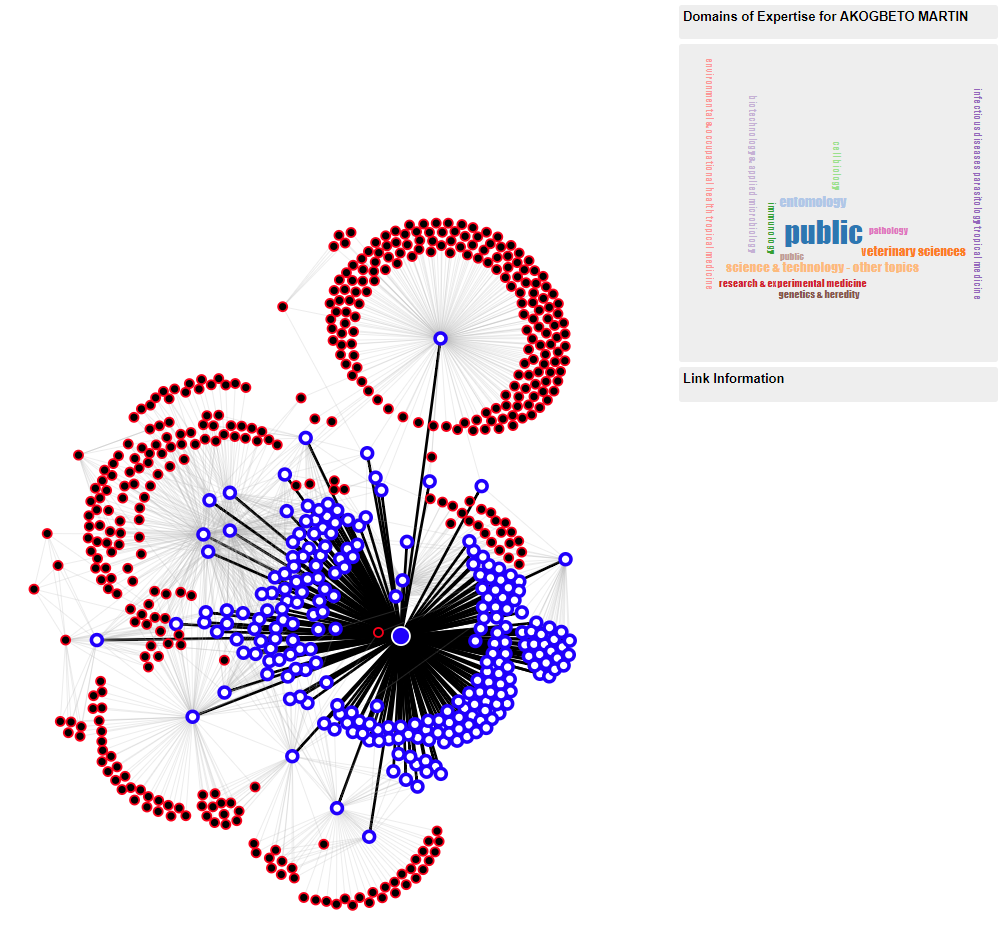
\includegraphics[scale=0.5]{Chapters/authorvis/mostCited}
\caption{Co-authorship network of the top 10 most cited papers in Malaria research in Benin.}
\label{mostCited}
\end{figure}
%%%

%is built using the Javascript library D3.js \cite{bostock_d3._2012}. The javascript library D3.js or Data-Driven Documents has been designed for manipulating documents based on data and to generate interactive and dynamic data visualizations in web browsers. 
%We built in a panel allowing the user to interact with the network and control physics of network \cite{newman_physics_2008}. We incorporated several Javascript functions to design an intuitive and user friendly visualization interface. A mouse hover over a vertex displays a tooltip of details on the author represented by the vertex while a double-click on a vertex highlights the subnetwork of the identified network. We made edges clickable. Once an edge is clicked, the list of published materials co-authored by the two vertices defining the clicked edge is displayed in a panel on the right hand side. All published materials listed can be traced back to their publication page on the web via their DOI or the WOS accession number with a single click. Figure \ref{net_vis} is a screenshot of the visualization interface. In the left pane in figure \ref{net_vis}, the user can adjust the display of the network by modifying the default options of the control physics of the network. The pane on the right displays related information to the selected edge (in blue on figure \ref{net_vis}) on the visualized network (in the middle of the display).

%\subsection{Web Framework}
%The whole system is built into a Shiny dashboard thanks to the R package \textbf{Shinyboard} \cite{chang_shiny:_2017,chang_shinydashboard:_2015}. Using the dashboard, the user can choose to use the prediction tool menu, or query and visualize the network data. We also provide within the dashboard all our Shiny codes and a link to our Git directory containing all our source codes. \\
%The prediction tool is model based and used the final ERGMs from chapters 3, 4, and 5 to calculate a probability of collaboration between two authors. A micro-interpretation of the model is provided based on the user query  \cite{desmarais_micro-level_2012}. \\
%When the user chooses the visualization menu, an interface allows him to submit his query to the system. The query is interpreted and processed on the server end and the user is automatically prompted to a new visualization page.

\section{Deployment}
The system is packed in a Docker container to facilitate its use and installation. The docker container is accessible at \url{https://hub.docker.com/r/rosericazondekon/authorvis/}. The project source files can be forked or cloned from Github at \url{https://github.com/rosericazondekon/authorvis}. %We also made it accessible online via an  \href{https://#}{AWS server}.

%\section{Future Directions}
%Currently, \textbf{AuthorVis} is specifically built for Malaria, TB and HIV/AIDS in Benin. Future development will extend the tool to other research domain. We also aim at adding a general purpose module to \textbf{AuthorVis} for the visualization of any user-input co-authorship network. This will also require the integration of a data pre-processing module to facilitate the disambiguation and deduplication of co-authorship information. Finally, we will also incorporate a layered structured network visualization \cite{nakazono_nel_2006} functionality to the visualization in order to display temporal changes in the evolution of the co-authorship network.


%\section{Conclusion}
%Text for this section goes here...